\section{Results}
\label{sec:results}

The primary experiment is the Class~A search for a drifting, unresolved
spectral carrier: \NWinA{} fine-channel windows toward \NSysClassA{} systems,
\EdrNWinA{} of which are channelised finely enough on the criterion of
\S\ref{sec:statistic} to tell a drifting carrier from a stationary one. The
Class~B search for an unresolved spectral excess is secondary and carries no
drift discrimination: \NWinB{} coarse windows. Together they are the
\NWindows{} windows of the primary census. No event satisfied the confirmation
criterion set out in \S\ref{sec:summary}.

\subsection{Sensitivity: the power at which a carrier would have crossed
the threshold} \label{sec:pninetysel}

\emph{The median system, on its best window, would have produced a threshold
crossing from a carrier of $\EirpNinetySysMedA$\,W.} A limit is a statement
about bandwidth a carrier could have been reported in, so each window's limit
is taken over the channels the attribution mask leaves, in the star's own rest
frame (\S\ref{sec:summary}): the finest windows were tuned to CO, a
\UmFineChanKHz\,kHz window spans \UmFineBwMHz\,MHz against a mask
\UmFineMaskMHz\,MHz wide, and \UmNWinAFull{} of the \NWinA{} Class~A windows
therefore lie wholly inside it and constrain nothing, among them the two finest
in the survey. Across the \NSysALim{} systems left with a constrained window
those limits run from $\EirpNinetySysLoA$ to $\EirpNinetySysHiA$\,W
(Fig.~\ref{fig:classasens}a), \NSysEfifteen{} of them reach $10^{15}$\,W and
the median Class~A \emph{window} reaches $\EirpNinetyWinMedA$\,W, while for
\NSysALostName{} every fine window is inside the mask and no limit is quoted.
Over the \EdrNWinA{} windows in which the searched drift crosses a channel the
search covers \EdrUnionGHz\,GHz toward \EdrNSys{} systems, and their median
system limit is \ScEdrMedPct{} per cent \ScEdrMedSense{} than that.

\emph{They are a recovery completeness of one epoch, and not a threshold.}
Artificial carriers were injected at a random sub-channel phase and a random
drift from each window's own grid, then recovered through the unchanged
pipeline; the power at which nine in ten come back is $\mathrm{EIRP}_{90}$, the
only sensitivity quoted here, measured through the single-epoch trigger and the
localisation at the stellar position inside one execution block. It is
therefore the power at which a carrier would have produced a crossing and not
the power at which one would have been confirmed, because confirmation needs a
second and separated epoch, which the archive supplies for some systems and not
others (\S\ref{sec:mmdifferent}). The \NCtrl-position spatial rank decides
nothing and is not charged against it either: charging it would cost a further
factor $\SensCostLike$, and in \SensNRingHiUnres{} bright-ring windows it could
not be met at any injected power (Fig.~\ref{fig:strata}).

\emph{Measured that way the completeness is one number for the class.} Nine
carriers in ten are recovered at $\EirpNinetyMultA\,P_{\rm trig}$, with a
sampling error of $\pm\SensBootPct$ per cent on that pooled value -- a
statement about the class average and about no individual window -- against a
nominal threshold, $P_{\rm trig}$ being the bare $\LtCommonSnr\sigma$ of the
window itself. The loss a channel-confined carrier suffers to the correlator's
spectral response is carried by the injected tones, so it sits inside the
measured factor, $\times\RpRespFac$ of it, and is not applied to the result as
well (Appendix~\ref{app:conventions}). Every one of the \SensNInj{} directly
injected Class~A windows resolves a ninety per cent point of its own, and the
value does not depend on the brightness of its control ring
(Fig.~\ref{fig:strata}). Class~B carries its own factor $\EirpNinetyMultB\,P_{\rm
trig}$, which sets the limits for Barnard's Star, Wolf~359 and Proxima,
measured the same way from \SensNToneCoarse{} carriers injected into
\SensNInjCoarse{} coarse windows of \SensNInjCoarseBlock{} execution
blocks. Calibration of the class factor is good to
$\times\SensFacLo$--$\times\SensFacHi$ (Table~\ref{tab:p90budget}), an interval
on the median and on the counts and not on any one window's limit: the median
system's limit above carries it, $\TfMedCalLo$ to $\TfMedCalHi$\,W, so the
second figure of that median is set by the calibration and not by the depth of
any observation.

\emph{Every limit quoted here is nominal in one respect: it excludes
atmospheric decorrelation.} An injected carrier is added to already calibrated
visibilities and so suffers none, whereas a real carrier does, and the bias
runs one way only. Measured block by block from the phase rms the observatory
records on each block's phase calibrator \citep[\S\S10.4.11,
11.3.1]{ALMAHandbook} through the standard phase-scatter relation
\citep[Eq.~3]{Richards2022}, it leaves the median limit optimistic by
\SensDecorPct{} per cent and the median window above \SensDecorHiGHz\,GHz by
\SensDecorHiPct{} per cent. \emph{That is why this term is stated and not
folded in}: the factors that are applied are available for every window of the
census, while this one is available for \SensDecorNBlk{} blocks of
\SensDecorNBlkTot{} and the rest are measurably the harder ones, so folding it
in where it is known would leave a set of limits that is neither corrected nor
uncorrected. Table~\ref{tab:persys} gives it system by system
(Appendix~\ref{app:persys}).

Three further factors act window by window and are divided out of the limits
above rather than quoted beside them -- the primary-beam response at the star's
own offset from the pointing centre, the annual parallax the search's phase
centre omits, and the smearing of a carrier that sweeps within a channel during
one integration while an injected one does not -- each with its range and its
direction in Table~\ref{tab:p90budget}, its definition in
Appendix~\ref{app:conventions} or Appendix~\ref{app:pbresp}, and its own value
for every window in the released per-window catalogue. \emph{The net bias on
one window's
limit is therefore of either sign}: in the median window the injected profile's
\InjShortPct{} per cent shortfall against the exact channel response is the
larger term and the quoted limit is conservative by \NmNetConsPct{} per cent,
while at the ninetieth percentile of the systems' own best windows the
decorrelation is, and the limit is optimistic by \NmNetOptPct{} per cent,
rising to \NmNetOptMaxPct{} per cent for the most affected system.

\emph{Carriers were injected directly into \SensNInj{} of the \NWinA{} Class~A
windows, \SensNInjPct{} per cent, and the result transferred to the remaining
\SensNTransfer. That transfer is the dominant caveat on everything above.} The
injected windows are the Class~A windows of execution blocks drawn in a random
order and balanced by band and array -- \emph{the unit is the block and not the
window}, because a block's calibrated visibilities are what an injection
campaign has to rebuild -- and over \RpNAxis{} properties, among them the
channel width, the integration time, the noise and the control-ring brightness,
they span the central eight-tenths of the population, five of the six agreeing
in the median to \RpCovOtherPct{} per cent and the sixth, \RpCovWorstAxis,
$\times\RpCovWorstRatio$ noisier, which follows from drawing whole blocks
(Appendix~\ref{app:persys}). What is carried across is one dimensionless number
per class, the ninety per cent point in units of the window's own trigger
power, while the channel width, the noise, the integration time, the
primary-beam response, the parallax displacement and the intra-integration
retention that turn it into a power are each that window's own
measurement. Across the injected windows that point ranges from
$\times\SensIndivFacLo$ to $\times\SensIndivFacHi$ of the adopted factor, with
\NmDispNTenth{} of the \SensNInj{} within a tenth of it, and \emph{that
dispersion, and not the calibration interval above, is what one uninjected
window's own limit is uncertain by}. Two bands and two channelisations hold no
injected window at all, \NgNExtrapWin{} windows between them, and
\NgExtrapTakeClause{} -- \NgExtrapSys{} -- so in each such case the
completeness is carried across a configuration boundary and the range just
quoted is not an empirical bound on it. The best window was
itself injected into for \SmcNMeasSys{} of the \NSysALim{} systems, marked as
measured in Table~\ref{tab:persys}; for the other \SmcNEstSys{} the headline
limit is an estimate carrying that dispersion.

\emph{A carrier that is not always radiating is penalised in proportion}: over
\DutyNTrial{} trials at duty cycles down to \DutyCycleMinPct{} per cent the
recovered amplitude followed the duty cycle to \DutyAttenDevPct{} per cent, so
a transmitter radiating a tenth of the time needs $\DutyPowFac\times$ the power
quoted above; those trials carry no drift, so the joint drifting and
intermittent case is not measured here.

\begin{table*}
\centering
\scriptsize
\caption{What sets $\mathrm{EIRP}_{90}$, and in which direction. The
calibration interval applies to the class-average factor and so to any
statistic over many windows; the spread between windows is an observed
dispersion and is the statement about one window; the signed terms are biases
and are not folded into an error bar (\S\ref{sec:pninetysel}).}
\label{tab:p90budget}
\setlength{\tabcolsep}{2pt}
% GENERATED by sens_r11.py -- do not hand-edit.
\begin{tabular}{@{}l@{~~}r@{~~}>{\raggedright\arraybackslash}p{0.61\linewidth}@{}}
\hline
 & value & what it does to the limit \\
\hline
Class-average completeness & $\times3.03$ & nine carriers in ten recovered at this multiple of a window's own trigger power. \emph{Measured} in the 49 Class~A windows injected directly and \emph{estimated}, at this factor, in the other 356 \\
\hline
\multicolumn{3}{@{}l}{\emph{Uncertainty on that calibration} (per cent), combined in quadrature} \\
The factor itself & $\pm2$ & sampling error of the pooled value over the 49 injected windows \\
Absolute flux scale & $\pm\BudFlux$ & the observatory's own band-dependent specification (\BudFluxSource): \BudFluxSpec, weighted over this sample's bands \\
Distance and visibility scale & $\pm\BudDistVis$ & the Gaia parallaxes, which enter as $d^{2}$, and the block-to-block visibility scale \\
\emph{Combined} & $-11/+11$ & $\times0.89$--$\times1.11$ on the factor, and so on the median limit and on the system counts; $\pm\BudCombWorst$ for the \BudNHiWin{} Class~A windows in \BudHiBandWord~\BudHiBands, at \BudHiGHzList\,GHz \\
\hline
\multicolumn{3}{@{}l}{\emph{Spread between windows}. An observed dispersion, not an error bar.} \\
Window to window & $\times0.80$--$\times1.58$ & the 49 injected windows resolve 2.41--4.80\,$P_{\rm trig}$ individually, \NmDispNTenth{} of them within a tenth of the pooled value and the second largest at $\times\NmDispSecond$. This, and not the interval above, is what an estimated limit is uncertain by; it is wider, and it applies to \SmcNEstSys{} of the \NSysALim{} systems \\
\hline
\multicolumn{3}{@{}l}{\emph{Applied} window by window where a record allows it and bounded where none does, and so not combined with the above.} \\
Intra-integration smearing & $\times1.00$--$\times\SmcFacWorst$ & a carrier sweeps through part of a channel within one integration and the injected ones do not: $\eta_{\rm smear}$ at the drift that sets a ninety per cent point, from each window's own integration length where it is recorded (\SmcNMeas{} windows) and from the longest delivered anywhere where it is not (\SmcNBound) \\
Primary beam & $\times1.00$--$\times\NmBeamFacWorst$ & the star is not at the pointing centre, so each limit is divided by the response at its own offset, on the full width the observatory documents. Nothing in the median window; the \BmNAboveTenPct{} windows furthest off-axis carry the departure of that form from a blocked circular aperture, up to \BmModelMaxPct{} per cent, as a one-sided systematic \\
Annual parallax & $\times1.00$--$\times2.06$ & the phase centre omits it, so each limit is divided by the amplitude a compact source retains at its own displacement, a median \PxaLossMedPct\,per cent on the \PxaNWin{} windows carrying a parallax record; on the other \PxaNMissing{} the loss is bounded (Appendix~\ref{app:pbresp}) \\
\hline
\multicolumn{3}{@{}l}{\emph{Signed terms}. A bias is not an error bar and is not added to one.} \\
Channel response & $\times\RpRespFac$ & the share of a channel-confined carrier the peak channel keeps. Carried by the injections, so already inside the completeness above, which is this factor times a margin of $\times\RpMarginNinety$ over the nominal trigger \\
\quad its residual & $+\InjShortPct$ & the injected profile falls short of the exact response: \emph{conservative} \\
Decorrelation & $+0/+\SensDecorPct$ & measured block by block from the phase rms the observatory records on each block's phase calibrator, which an injected carrier does not suffer and a real one does: $+\SensDecorHiPct$ above \SensDecorHiGHz\,GHz, and more than $+\SensDecorTailLevelPct$ in \SensDecorTailPct{} per cent of windows \\
\hline
\end{tabular}

\end{table*}

\begin{figure}
\centering
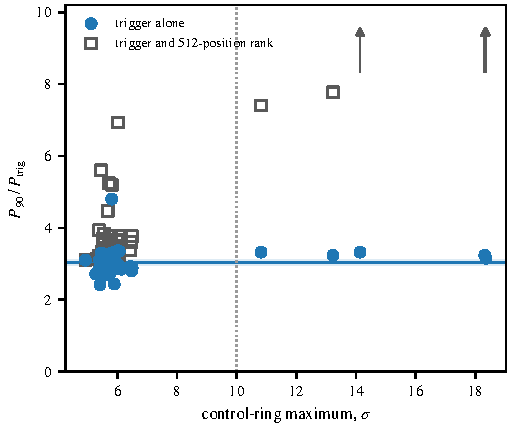
\includegraphics[width=\columnwidth]{figures/sens_ring.pdf}
%% ★ v4.26 (r25-captions): 9 printed lines -> R1 §7's limit of about six.
%% \S\ref{sec:pninetysel} above already carries every statement removed:
%% that the value does not depend on the ring's brightness, what charging
%% the rank would cost, and the bright-ring windows that cannot meet it at
%% any injected power -- the arrows.  \SensRingRule had this caption as its
%% only citation site, so the dotted line's threshold MOVED into that
%% paragraph rather than being dropped.
\caption{Why one completeness factor serves the whole class. The
\SensNInj{} directly injected Class~A windows at the power recovering nine
carriers in ten, each against its own \NCtrl-position ring maximum: no trend
with the ring. Filled, the criterion adopted here, pooled value as line and
band; open, the rank charged too, arrows where no power meets it; dotted, a
resolved ring.}
\label{fig:strata}
\end{figure}

\begin{figure*}
\centering
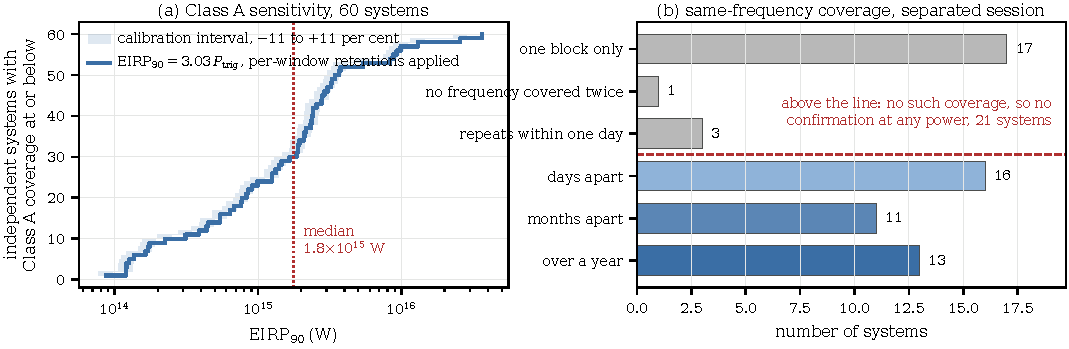
\includegraphics[width=\textwidth]{figures/classa_sensitivity.pdf}
%% ★ v4.26 (r25-captions): 9 printed lines -> R1 §7's limit of about six.
%% DELETED as said elsewhere and verified before deleting: "for an
%% accelerating carrier, confirmation further requires the repeat to fall at
%% a matching orbital phase" stands in Fig.~\ref{fig:confcov}'s caption AND in
%% \S\ref{sec:confirmability}; the grouping over "the primary census together
%% with every repeat block the recurrence test reads" is
%% \S\ref{sec:confirmability}'s own sentence; and the closing paragraph
%% re-states that section's opening line, "a sensitivity limit and a
%% confirmation limit are different statements", which is kept here in one
%% clause because it is what the figure is for.  No macro lost a site.
\caption{\textbf{The two completenesses of the carrier search, over the same
\NSysClassA{} systems}, which are separate statements and neither of which
follows from the other (\S\ref{sec:mmdifferent}).
\emph{(a)}~Single-epoch trigger completeness: the cumulative number of
systems whose best window reaches a given $\mathrm{EIRP}_{90}$, each
window's own retentions applied and atmospheric decorrelation excluded
(Table~\ref{tab:p90budget}, whose calibration interval is the shaded band).
\emph{(b)}~Systems with same-frequency coverage in a separated session,
which no amount of power buys, grouped by the longest separation between two
such sessions. \textbf{Left of the dashed line, \ZcNoRepSys{} systems have
no such pair, and for them confirmation was not possible at any sensitivity
in panel~(a)}.}
\label{fig:classasens}
\end{figure*}

\subsection{The nearest stars: Barnard's Star and Wolf~359}
\label{sec:barnardswolf}

Barnard's Star is the second-nearest stellar system and Wolf~359 the third if
brown dwarfs are excluded, and to our knowledge these are the first millimetre
or submillimetre technosignature limits for either; radio searches of the
nearest stars have worked at centimetre wavelengths
\citep{Enriquez2017,Price2020,Margot2023}. Both are non-detections, and
\emph{both limits come from the secondary Class~B experiment and not from the
carrier search}, the archive holding only coarse Band~6 windows toward these
stars: on the $\mathrm{EIRP}_{90}$ convention of \S\ref{sec:pninetysel}
Barnard's Star reaches $\EirpNinetyBarnLo$--$\EirpNinetyBarnHi$\,W over
\NWinBarn{} windows and Wolf~359 $\EirpNinetyWolfLo$--$\EirpNinetyWolfHi$\,W
over \NWinWolf.

\subsection{Threshold crossings and how each was disposed of}
\label{sec:technosearch}

\emph{The result is a chain of three tests, and it is read in one direction.}
Of the windows the search covers -- the \NWindows{} of the primary census and
the archival-tail blocks beside them -- \EvNCrossRaw{} hold a cell reaching
$T\geq5$ at the stellar position. \EvNCrossFlag{} lie in the one execution
block that fails the quality criterion of \S\ref{sec:bdblock}, so the
population that characterises the search is the \EvNCrossQp{} in
quality-passing data and those \EvNCrossFlag{} are reported beside it. The
molecular-line mask is $\pm\MaskHalfKms$\,km\,s$^{-1}$ wide in each star's own
rest frame and places \MkNCoinc{} of the \EvNCrossQp{} within that distance of
a catalogued transition; a further \SoNCrossWord{} fall on transitions of a
species no debris disc has been shown to carry, which the mask does not hold,
and stay unattributed with their offsets reported
(Appendix~\ref{app:linemask}). That leaves \EvNAttrQp{} crossings attributed
and \EvNUnattrQp{} unattributed, and the attributions are kinematic and not an
accident of bandwidth: in the frame the correlator delivered, the crossings
with a measured peak frequency crowd onto the transitions these setups were
tuned to far more tightly than a free landing on their own grids would put them
(Appendix~\ref{app:rfi}). Of the unattributed, \EvNRankQp{} outrank all
\NCtrl{} control positions of their own window, and none was found again in any
other epoch covering its frequency. No crossing survives the chain, and this
survey reports no detection; the crossing ledger, which accompanies this paper
as data, lists every one.

\emph{Anything bright in a window hides a weaker carrier behind it, so the
weaker cells were sought too.} The de-drifted statistic is retained in every
channel, so behind a window's tabulated crossing -- its largest cell -- weaker
above-trigger cells can be read as well, neighbouring channels counting as one:
there are \CkNSecondaryWord{} of them, of which \CkNSecUnattrWord{} are
unattributed and \CkNRecurWord{} reaches the trigger in any of the covering
blocks the recurrence test reads. Cells are counted in the controls too, and
outside the mask the star holds slightly more of them than a control position
at every level below the trigger, with no step where a carrier search would put
one (Appendix~\ref{app:falsealarm}, \S\ref{sec:trigunif}).

\subsubsection{The unattributed count is what the control positions predict}
\label{sec:trigunif}

The trigger is a threshold on a statistic and not a false-alarm rate: the
number of searched channel\,$\times$\,drift cells per window spans
\TuCellsDecades{} decades, so one level buys very unequal protection. How
many crossings chance should produce is therefore measured window by window,
over the \CeNWin{} Class~A windows of the census and with one condition on
both sides of the comparison: a cell at the stellar position that reaches the
trigger and that the line mask does not attribute. Both quantities are read from the data themselves, and
Appendix~\ref{app:falsealarm} gives that accounting. The control positions carry no continuum, so a calibration error varying
with frequency would raise the star and not them; on the continuum these
stars have, the least demanding window would need
\CyEpsMinPct{} per cent of it to reach the trigger, and the mild excess of
\S\ref{sec:technosearch} runs the wrong way with continuum brightness,
\CkRatioContBright{} against \CkRatioContFaint{} over the \CkNContWin{}
windows with a photospheric estimate (Appendix~\ref{app:radius}). These fields' own control positions predict \CeExp{} unattributed
Class~A crossings and \CeObs{} are found. A count that large or larger arises
by chance with probability \CeProbNull{} -- a probability conditional on the
control positions being a model of the stellar position, which is the one
assumption the searched data cannot test. Calibrating the stellar rate
against the control rate instead, as a sensitivity test at the ratio
\CeNear{} measured just below the trigger, gives \CeExpNear{} expected at
$P=\CeProbNear$, and the conclusion of no significant excess is unchanged
under it; the control positions' own rate is adopted as the more demanding of
the two (Appendix~\ref{app:falsealarm}). Both sides are read over the whole
primary beam \S\ref{sec:statistic} defines, and that is the reading the
abstract and \S\ref{sec:summary} quote -- not because it was nominated
first, but because it is the statistic Equation~\ref{eq:tstar} specifies,
whereas a narrower field drops the integrations whose pointing falls outside
it and with them on-source time and real signal. Read over such a field on
both sides the same comparison gives \FrNarrowObs{} against \FrNarrowExp{}
at $P=\FrNarrowProb$, reported beside the first and not in place of it. Both
are extraction geometries applied uniformly to every window and to both
sides, so neither was defined by reference to the counts -- but neither was
nominated as the primary before the counts were compared, and the choice
between them was made after the counts had been seen. The whole beam shows no
significant excess and the narrower field a nominal one; with \FrNRead{}
readings tested the smaller of the two probabilities, corrected for
\FrNRead{} trials, is \FrTwoTrialP, so neither departs from chance at the
\CeAlphaPct{} per cent level. That correction does not settle the
disagreement between them, since it assumes the analysis involved only these
\FrNRead{} choices. The interpretation therefore depends to some extent on
the extraction geometry, and neither reading establishes a population of
non-astrophysical transmitters. The two disagree on \FrNFlag{} of the
\CeNWin{} windows and in both directions: the whole beam holds a crossing the
narrower field does not toward \FrUpStars, both of them attributed to carbon
monoxide, and the narrower field holds one the whole beam does not toward
\FrDownStars. The stars do carry more above-threshold cells than their own
controls below the trigger, and that excess has no identified cause; the rate
adopted is the control positions' own, and
Appendix~\ref{app:falsealarm} gives both readings and carries the excess
as a sensitivity test. A further \CeNTailCrossWord{} unattributed
crossings, both toward \CeTailStar, lie in archival-tail blocks the catalogue
does not tabulate window by window, and enter neither side.

The observed count is therefore compatible with a background estimated
empirically from these same fields, and that is not the same thing as a null
distribution established independently of the model: the attribution applied
to both sides, one count per window, and the control positions' own rates.
What this comparison could not have rejected is \CeAddLim{} further
crossings against those same control positions, \FrNarrowAddLim{} on the
narrower reading -- conditional on that model, a count of crossings and not
of transmitting systems, since several crossings could come from one source,
not an occurrence rate, and not a statement about technosignatures of any
other kind (Appendix~\ref{app:falsealarm}). Each
crossing is tested individually by the recurrence test of
\S\ref{sec:etacrv}.

\subsubsection{One execution block accounts for four of the crossings}
\label{sec:bdblock}

\BdNCross{} crossings belong to \BdStar{} (\BdAlias), all of them in one ACA
execution block, \texttt{\BdBlock}, whose whole field is above threshold:
\BdNCtrlAbove{} of its \BdNCtrl{} control positions exceed $T=5$, where the
median of a window's own control ensemble is \BdSurvCtrlMed{} across the
survey. Its
single-integration noise is as predicted but it does not integrate down, a
jackknife on the channel mean standing \BdJackRatio{} times above thermal while
neighbouring channels stay uncorrelated, which describes a residual persisting
from one integration to the next and differing from channel to channel
(Appendix~\ref{sec:blockquality}). Equation~\ref{eq:tstar} divides by the noise
of the stacked spectrum, which falls as the root of the integration count, so a
residual that does not average down accumulates along a drift track faster than
the denominator grows, and it does so at every position in the field.
\emph{The field is inflated and the star is not}: the \BdNSibling{} sibling
executions of the same field, array and setup produce no crossing, and in the
strongest of the four more than a tenth of the \BdNCtrl{} controls stand above
the star. The criterion fails this block and no other at any threshold between
it and the next most extreme block, so its \BdNCross{} crossings are reported
apart from the \EvNCrossQp{} and Appendix~\ref{app:rfi} carries what the block
might instead be. Milder cases are not unique to it: read window by window the
same diagnostic flags \DqNWin{} windows in \BkFlagNBlock{} blocks, and the
\BkFlagNCrossOther{} flagged crossing outside this block -- \BkFlagOtherStar{}
-- is withheld from the amplitude-dependent tests for it too.

\subsubsection{Stellar flares are excluded by a broadband prediction}

Known flare stars are in the sample, but a millimetre flare raises every
channel of a window alike, so one able to produce a single-channel crossing at
the trigger must produce a $5\sqrt{N}\sigma$ continuum event in the same
integrations: with $N$ the window's own channel count,
\FlNChanLo--\FlNChanHi{} across the windows holding a crossing, that prediction
runs \FlPredLo--\FlPredHi$\sigma$, against an observed continuum statistic of
median \FlObsMed{} over the \FlNCont{} crossings with a recoverable measurement
and $|Z|<3$ in \FlNQuiet{} of them. A flare origin in fact needs more than
that, because the per-integration median along frequency
(\S\ref{sec:statistic}) removes a flat continuum before the search: only a
flare's departure from flatness across the band can reach a single channel, so
the prediction is a floor on what such an origin requires and the contribution
measured below is a bound on what one supplies. One block settles it:
\FlEgStar{} \texttt{\FlEgEb} holds both a crossing ($T_\star=\FlEgT$) and the
millimetre flare of \citet{MacGregor2020}, and that flare contributes
\FlEgContrib$\sigma$ to the single-channel statistic -- raising the continuum
at $Z=\FlEgContZ$ while the crossing's own de-drifted track reaches
$Z_{\max}=\FlEgTrackZ$.

\subsection{$\beta$~Pictoris: an astrophysical positive control, and the
obstacle it identifies} \label{sec:bpicval}

\emph{A search that finds nothing must show that it could have found something,
and the survey's strongest features show exactly that.} The pipeline recovers
the $\beta$~Pictoris circumstellar carbon monoxide without being told the disc
is there, in two rotational transitions and in \CsBpCoBlocks{} execution blocks
spanning \BpBaselineYr\,yr drawn from \CsBpCoSess{} observing sessions, the
closest two \CsBpCoSepMinD\,d apart; in \NStageOneBpicEb{} of the blocks the
star also outranks every control, but the identification is kinematic and does
not rest on those statistics -- carried through the frame chain to the
barycentre at each block's own epoch and then to the star's rest frame, all
\BpicPanelNCo{} crossings lie within \BpicDvCoHi\,km\,s$^{-1}$ of the stellar
systemic velocity, in the two lowest CO transitions of a star with mapped
circumstellar CO \citep{Dent2014,Matra2017}, and the Band~3 peaks agree across
blocks to \BpRecThreeTuneChanMax{} channel once each block's own tuning is
removed. The alternative reading requires a transmitter placed by coincidence
at matched offsets from two CO transitions of one star. It is also the control
that shows the recurrence test of \S\ref{sec:etacrv} working in the positive
direction: every flagged feature is recovered in another execution block and
each transition in a block of another session as well, the screened Band~6
window returning $T_\star=\BpRecTTwo{}$ -- and a non-recurrence elsewhere means
nothing unless the same machinery recovers a repeat where one exists.
\emph{One of those blocks is a counterexample, and it is the more useful half of
the control}: in block \texttt{\BpCtrlBlock}, Band~\BpCtrlBand, the control ring
reaches \BpCtrlRingMax{} against \BpCtrlStar{} at the star, so several of the
\NCtrl{} control positions exceed the stellar statistic and the spatial rank
disfavours a window holding carbon monoxide known to be real and centred on the
star. The disc is resolved on the scale of the primary beam in that
configuration, which is the geometry the statistic is built to reject, so the
rank is a test of compactness and not of authenticity and on a real extended
source it errs conservatively -- a stronger statement than a clean positive
control, because it bounds the diagnostic's reach as well as demonstrating it
(Fig.~\ref{fig:bpiccontrol}). Extended emission is in fact identified by the
\emph{level} of the control ring and not by the star's rank against it, which
is why the window-level flag of Appendix~\ref{sec:blockquality} is defined on
the ring's median, and Appendix~\ref{app:linemask} gives the complementary case,
HD~48370, whose crossing matches the prominent CO($2{\to}1$) that
\citet{Cataldi2023} report toward the source and flag as possible cloud
contamination, and whose control ring rises with the star as emission filling
the primary beam does. The mask that removes
this emission covers \FrNSpec{} species and costs \MkMaskAPct{} per cent of the
Class~A union bandwidth, and it is nevertheless the single most productive test
in the chain (Appendix~\ref{app:linemask}); \S\ref{sec:mmdifferent} draws the
lesson.

\subsection{The two crossings that lead their own control fields}
\label{sec:vistest}

Frequencies in this section and the next are in the star's own rest frame,
which is the frame the recurrence test registers in; the delivered ones are in
Table~\ref{tab:cand} and in the ledger. Two crossings reach a stellar statistic
above every one of the \NCtrl{} control positions in their own window, and
neither is a detection: \EvAStar{} at \RqFreqSx\,GHz and \EvBStar{} at
\RqFreqCp\,GHz, both in Band~\EvABand, tabulated in Table~\ref{tab:cand} and
the first drawn in Fig.~\ref{fig:event}. Their control rank is recorded because
it says which crossing was examined first, and it disposes of nothing
(\S\ref{sec:method}). Were the stellar and control positions exchangeable, the
star would lead all \NCtrl{} of them with probability $1/\RkCtrlDen$, so
\RkExpLead{} of the \RkNUnattr{} unattributed crossings would do so by chance
and two or more with probability \RkProbTwo, against \RkHoLead{} of \RkHoN{} in
the reserved blocks and \RkOosLead{} of \RkOosN{} beyond 40\,pc. That the two
observed are unlikely on that model is not evidence of a signal, because the
two sets of positions are not exchangeable (\S\ref{sec:summary}) and neither
crossing recurs. \EvBStar's crossing lies $\EvBDv$\,km\,s$^{-1}$ from \EvBLine,
a coincidence reported as a note and not as a disposition
(Appendix~\ref{app:linemask}). Each was re-fitted in the visibility domain, as
\LgNFit{} of the \NCross{} crossings were, by phase rotating to the star and
following the recovered drift, and \LgNLocalCor{} of those fits are consistent
with a point source at the star; the fit excludes neither crossing, because
injected sources in the bin these two occupy return ${\rm
Re}/\sigma=\RsevReAtFiveMeanA\pm\RsevReAtFiveSdA$, and its value is that a
pedestal fed through a sidelobe from elsewhere in the field -- which a dirty
map at the star cannot tell from a source at the phase centre -- is not a point
source there. Of the \NCtrl{} control positions the rank screen uses,
\RcNRetCtrl{} retain a dynamic spectrum and \RcNVisCtrl{} are reachable in the
visibilities.

Neither crossing is present when the same stellar-frame frequency is observed
again, and Table~\ref{tab:cand} gives both readings of that silence: the
nearest covering block assumes least, lying \RcSxNearH{} and \EvBDeepH\,hours
from each discovery and ruling out anything above \RqNearFracSx{} and
\RqNearFracCp{} of the discovery amplitude, while combining every covering
block deepens that to \RcSxFive{} and \RcCpFive{} but asks the same return over
baselines of \RqSpanDSx{} and \RqSpanDCp\,days rather than of hours. Either
reading covers half a channel in the star's frame, $\pm\RqDispSx$ and
$\pm\RqDispCp$\,km\,s$^{-1}$, which each carrier's own fitted drift would cross
in \ZtSxLeaveSec{} and \ZtCpLeaveSec{} seconds: the test asks for a return to
that frequency, not a stability at it (\S\ref{sec:etacrv}), and
Table~\ref{tab:cand} reports both as the statistic a carrier persisting at the
discovery amplitude would have given at the predicted stellar-frame cell,
$T_{\rm pers}$, against the $T_{\rm rep}$ measured there. That reading is one
cell at one trial and so may be negative, where each indented reading beneath
it is a maximum and so positive on average whatever is present, and the same
chance computed at the discovery amplitude itself, which Table~\ref{tab:cand}
gives in brackets, is biased high. At the faintest amplitude consistent with
each crossing having been found at all the criterion would have recovered a
persisting carrier with calculated probability \RqPowerTrigSx{} and
\RqPowerTrigCp, and injected carriers at that amplitude are measured at
\HjMeasSx{} and \HjMeasCp{} in the accompanying data -- so for \EvBStar{} the
silence is not an exclusion and is not read as one. Appendix~\ref{app:radius}
follows its crossing through every step of the chain.


\subsection{Recurrence, applied to every unattributed crossing}
\label{sec:etacrv}

A transmitter on a body in orbit about its star does not arrive at the same
frequency twice: its line-of-sight velocity changes between epochs, and a
carrier at a fixed rest frequency changes with it. The question the repeat
coverage can answer about such a carrier is therefore the broad one --
whether anything above the trigger is present again anywhere in a covering
window, searched at every drift of the grid -- and it is the result this
section leads with. That window is $\pm\WdHalfKms$\,km\,s$^{-1}$ wide in the
median case, against the $\pm\EcVexcKms$\,km\,s$^{-1}$ an orbit at the grid's
own \WdAGrid\,m\,s$^{-2}$ ceiling can produce about any star in this sample,
whatever its eccentricity and orientation, so it spans the excursion such a
carrier could have made. \WuNWinExc{} of the \WuNWin{} distinct covering windows hold a
statistic above the trigger, against the \WuExpWin{} chance predicts
($P=\WuProbWin$), and every one of those \WuNWinExc{} windows holds a
crossing the ledger already lists -- so this comparison re-reads the
trigger-level excess of \S\ref{sec:trigunif} over the same control positions
rather than adding a recurrence to it. \WuNWinExcTwo{} of the
\WuNWinExc{} are toward \WuTwoStars{} alone; over the remaining
\WuNWinRest{} windows the reading is \WuNWinRestExc{} against
\WuExpRest{} at $P=\WuProbRest$, so such departure as there is sits in two
objects and is not a property of the sample. That expectation is a sum of each
window's own
chance of holding one cell above the trigger, from its independent
channel--drift cells and the noise its own control positions measure, and
not a control rate applied to their number (Appendix~\ref{sec:pairacct}). The strongest of them reaches
\WdExcMax{} and the nearest sits \WdNearKms\,km\,s$^{-1}$ from the crossing's
own frequency, a median \WdMedKms\,km\,s$^{-1}$ away. A catalogued window
covers \WdNOrbTot{} of the \RcNExcl{} crossings that carry an amplitude
bound and spans that excursion in \EcNSpan{} of them; for \EcNShort, toward
\EcShortStarList, the widest covering window is narrower than the excursion,
and \WdNNoCov{} is covered by no catalogued window at all -- \WdNoCovStar,
whose one repeat reading comes from \texttt{\WdNoCovEb}, an uncatalogued
tail block \WdNoCovSepD\,d later. No recurrence
is established here, and none is excluded.

A carrier present again would appear in its repeat block as a crossing,
so each pair must be asked whether one transmitter could have produced both
members. Of the \TjNCandPair{} pairs inside that interval with at least one
unattributed member, Table~\ref{tab:pairs} asks the question of the \TjNPair{}
across \TjNStarPair{} stars whose two crossings each carry an independently
fitted drift and a block epoch measured from their own data; the other
\TjNCandLost{} want a discovery spectrum or a fitted drift
(Appendix~\ref{sec:pairacct}). Both fitted drifts are carried into the star's
frame first, by removing the observatory's own line-of-sight acceleration,
which is diurnal here and so cannot be extrapolated across days;
Table~\ref{tab:pairs} marks that frame with the subscript $\star$ and carries
the stellar-frame offset $\Delta\nu$ beside the two rates, while
Appendix~\ref{sec:edge} gives the rates in the observatory's frame, the frame
the grid is stepped in. Constant line-of-sight acceleration means
$\dot\nu_1=\dot\nu_2$, which \TjNUneqDrift{} of the \TjNPair{} pairs fail by
more than the grid resolves, and the \TjNPower{} pairs whose rates the grid
resolves fail a drift changing at a constant rate as well. The claim the
measurement supports is weaker and safer -- that no trajectory inside the
searched grid joins the two crossings -- and it separates \TjNExcl{} pair, the
two crossings of \EcGridStar{} needing \EcGridFactor{} times the grid's own
ceiling between them; Table~\ref{tab:pairs}'s \emph{Miss} column is that
departure in units of the drift grid's own resolution over $\Delta t$, and a
dash marks a pair the comparison has no power over at all. The other
\TjNOpen{} are unresolved, neither a confirmation nor an exclusion:
\TjNOpenPlain{} \emph{open} and \TjNPairEdge{} \emph{edge-limited}, where one
of the two fitted rates sits at the edge of the grid and is a lower bound. The
comparison has the power to reject, which it uses on all \TjNPower{} resolved
pairs, and none to accept a drifting carrier -- and it does accept the one pair
that is a single emitter, the \TjCtlLine{} line of \TjCtlStar, a line that does
not drift and which Table~\ref{tab:pairs} carries below its rule as a control
row.

\emph{A third reading is a check on line attribution, and not a test of
persistence.} The ledger also reads, for every crossing, the single cell its
own discovery predicts -- the stellar-frame frequency re-registered at the
repeat epoch, maximised over nothing. That cell is the right one for an
emitter at rest in the star's own frame, which is what a spectral line is, and
the wrong one for the carriers these crossings would be: every one of the
\RcNExcl{} has a fitted line-of-sight acceleration of \ZtALosLo{} to at least
\ZtALosHi\,m\,s$^{-2}$ in the observatory's frame and at least
\EgStarALosHi{} in the star's own, which carries a carrier out of the
half-channel the reading covers in \ZtSxLeaveSec{} to \ZtCpLeaveSec{}
seconds. It is therefore reported here as a \emph{line-recurrence check}, and
no crossing is called excluded on it. It works in that direction:
\MkAttrRecur{} of the \MkAttrTested{} crossings attributed to circumstellar or
interstellar carbon monoxide are present again -- \RqNRecurDisc{} in the
resolved disc of \RqRecurDiscStars{} and \RqNRecurCloud{} in interstellar gas
toward \RqRecurCloudStars{} (Appendix~\ref{app:linemask}) -- each recovered in
a block of another observing session more than \EpSep{} day from its own, the
strongest such recovery \QcSepMinD{} to \QcSepMaxD{} days away. Close to the
trigger the control is thinner than that count suggests: every circumstellar
recovery has $T_\star\ge\RqRecurDiscTLo$, and the \MkAttrExcl{} attributed
crossings not recovered are the two faintest tested, both at
$T_\star=\RqNearTrigT$ and both still consistent with their attribution, so
there the check rests on \RqRecurCloudStars{} alone. On the \RcNTested{}
unattributed crossings it returns nothing: none is present at its predicted
cell, the largest single-block reading at the carried drift being
\RcTMatched{} against a trigger of \StageNullTrig. What a null there bounds is
a carrier whose stellar-frame frequency is unchanged between the two epochs to
within half a channel and nothing wider; over the \RcNExcl{} crossings whose
repeat coverage carries an amplitude bound that bound reaches a median
\RcFracMed{} of the discovery amplitude and only \RcFracMax{} at the weak end,
where \HjNPowerLo{} of them are too shallow to test at the trigger
amplitude
(Appendices~\ref{sec:nullscatter}
and~\ref{sec:regbudget}, which also show that no disposition depends on the
registration of that cell, on the anchor along the discovery track or on the
threshold). Three statements come out of this, and they are not the same
statement: no crossing satisfies the confirmation criterion of
Table~\ref{tab:quantities}; the repeat coverage holds no excess of compatible
crossings over chance; and none of the three readings bears on a transmitter
whose apparent frequency or acceleration changes between epochs by more than
they accommodate.


\subsubsection{The reserved hold-out and the control beyond 40\,pc}
\label{sec:holdoutsearch}

Three sets of execution blocks enter no census statistic
(Table~\ref{tab:blockledger}); each was searched with the same pipeline and
each is reported here as a search. The \emph{hold-out} is \HoNBlock{} blocks,
\HoNWin{} windows, \HoNStar{} stars and \HoHours\,h on source, set aside by the
identifier rule of Appendix~\ref{sec:heldout} and sharing no execution block
with the census; it contains \HoNCross{} threshold crossings, the strongest at
$T_\star=\HoTMax$, none of them outranking its own control positions, and of
the \HoNTested{} tested for recurrence on the same code path exactly one is
present again -- a molecular line, so the test works in the positive direction
here as well, at $T_{\rm rep}=\HoRecTRep$ -- while for every other tested
crossing the repeat coverage rules out a carrier at \HoFracMax{} of the
discovery amplitude or less. The \emph{archival extension}'s \LdgExtWin{}
windows in \LdgExtEB{} blocks hold \QxObsCross{} threshold crossings, every one
in a fine-channel window, \QxObsAttr{} inside the mask in their own star's
frame and \QxObsUnattr{} outside it against \QxLam{} predicted by chance
(Appendix~\ref{app:falsealarm}), so the chance of \QxObsUnattr{} or more is
\QxPGe{} and a sample this size could have shown a shortfall and does not,
$P(0\,|\,\QxLam)=\QxPZero$. The \emph{control beyond 40\,pc} is \OosNBlock{}
blocks and \OosNWin{} windows toward \OosNStar{} background sources,
\OosHours\,h on source, holding \OosNCross{} crossings, the strongest at
$T_\star=\OosTMax$ and none outranking its own controls; \OosVsysClause, so the
set supports no limit and shows only that the pipeline behaves the same way on
fields beyond the sample. The hold-out crossings are released row by row with
the catalogue, on the columns of the crossing ledger.

\begin{figure*}
\centering
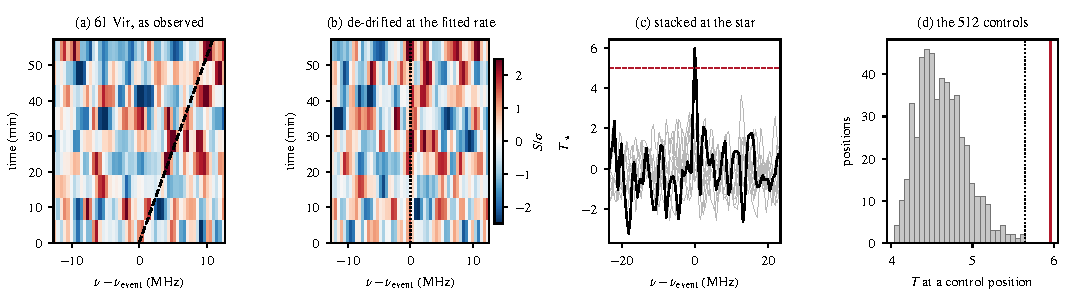
\includegraphics[width=\textwidth]{figures/event_crossings.pdf}
\caption{\textbf{The strongest unattributed crossing of the quality-passing
data, and the control field it leads.} Frequencies are in the star's rest
frame.
\emph{(a)}~The dynamic spectrum at \EvAStar's position around the crossing
at \RqFreqSx\,GHz, observed \EvADate, the fitted drift of
\EvADrift\,Hz\,s$^{-1}$ dashed, \EvANInt{} integrations binned into
\EvANBin{} and plotted in units of each bin's noise.
\emph{(b)}~The same rows shifted by that drift.
\emph{(c)}~The de-drifted stack at the star (black) and at the
\RcNRetCtrl{} control positions with retained dynamic spectra (grey), in
units of its own noise, the trigger dashed. \emph{(d)}~The same statistic at
each of the \NCtrl{} rank-screen control positions: the star (solid) against
the highest control (dotted).}
%% ★ v4.26 (r25-captions): 8 printed lines -> R1 §7's limit of about six.
%% MOVED into \S\ref{sec:vistest} above, carrying seven macros this caption
%% was the only citation site of (\EvAFlux, \EvAFluxErr, \EvARmsInt,
%% \EvAPerIntSig, \EvADwellMin, \EvADriftChan, \EvAChanwkHz,
%% \EvAElapsedMin): the per-integration significance and the drift's reach
%% across the block, both of which are statements about the crossing and not
%% keys to the panels.  DELETED: the closing pointer to
%% Table~\ref{tab:cand} and to \EvBStar{} at \RqFreqCp\,GHz, which
%% \S\ref{sec:vistest}'s own second paragraph states in the same words.
\label{fig:event}
\end{figure*}

\begin{table}
\centering
%% ★★★ v4.26 (r25-captions): 16 PRINTED LINES -> the author's limit.  Nothing
%% here was dropped on the floor: the $\pm\WdHalfKms$ interval and the
%% \TjNCandPair{} it holds are \S\ref{sec:etacrv}'s own second paragraph
%% already; \emph{edge} is defined there verbatim; and the subscript $\star$,
%% the observatory-frame pointer to Appendix~\ref{sec:edge} and the
%% \emph{Miss} column's units are now sentences in that same paragraph, which
%% is where a reader meets the table.  Measured with capmeasure.py.
\caption{\textbf{Can two crossings be one carrier?} The \TjNPair{} pairs
toward one star with an unattributed member. \emph{Miss}, the starred rates,
the control row and the verdicts: \S\ref{sec:etacrv}.}
\label{tab:pairs}
\scriptsize
%% GENERATED by pairs_v415.py -- do not hand-edit.
\begin{tabular}{@{}l@{~}l@{\hspace{4pt}}r@{\,}r@{\,}r@{\,}r@{\hspace{3.5pt}}r@{~}l@{}}
\hline
Star & blocks & $\Delta t$ & $\dot\nu_{1\star}$ & $\dot\nu_{2\star}$ & $\Delta\nu$ & miss & one \\
 & & (d) & \multicolumn{2}{c}{(Hz\,s$^{-1}$)} & (MHz) & ($\sigma$) & carrier? \\
\hline
61~Vir & X822/X82f & 3.00 & $+1092$ & $+3221$ & $+755.4$ & 15 & open \\
J1537$-$3319 & X10359/X398 & 123 & $-2000$ & $+2390$ & $+223.5$ & 3.6 & open \\
AU~Mic & X1838/X319 & 310 & $+1440$ & $+2645$ & $-159.0$ & -- & open \\
HD~14055 & X2b2ee/X2c3bb & 0.09 & $-2390$ & $+4216$ & $+825.2$ & 2447 & no \\
 & X24be0/Xd46 & 1.92 & $+1134$ & $-3823$ & $+63.0$ & 41 & open \\
 & X2c3bb/X3835 & 2.00 & $+4216$ & $+1800$ & $-514.6$ & 144 & edge \\
 & X2b2ee/X3835 & 2.09 & $-2390$ & $+1800$ & $+310.6$ & 48 & open \\
 & X3835/Xd526 & 607 & $+1800$ & $-2563$ & $-555.5$ & -- & open \\
 & X2b2ee/Xd526 & 609 & $-2390$ & $-2563$ & $-244.9$ & -- & open \\
 & X3835/X25c5e & 649 & $+1800$ & $+2611$ & $+423.3$ & -- & open \\
 & X2c3bb/X25c5e & 651 & $+4216$ & $+2611$ & $-91.3$ & -- & edge \\
 & X2b2ee/X25c5e & 651 & $-2390$ & $+2611$ & $+733.8$ & -- & open \\
$\beta$~Pic & X3a90/Xa9df & 1.02 & $-1611$ & $-679$ & $+85.5$ & 132 & open \\
\hline
HD~285968 & X108f/X5b4e & 4.99 & $-29$ & $-29$ & $-0.002$ & 0.6 & yes \\
\hline
\end{tabular}

\end{table}

\begin{table}
\centering
%% ★★★ v4.26 (r25-captions): 15 PRINTED LINES -> the author's limit.  The row
%% stubs of tab_recurcand_v411 already label $T_{\rm pers}$, $T_{\rm rep}$,
%% $(T_{\rm rep}+5)/T_{\rm pers}$ and the $\Phi$ rows in words, so the caption
%% was re-stating the table.  What was NOT anywhere else -- the sign of
%% $T_{\rm rep}$ against the indented maxima, and "in brackets the same at $S$,
%% which is biased high" -- is now \S\ref{sec:vistest}'s prose, two
%% paragraphs above this float.  The half-channel displacement is already in
%% that section ($\pm\RqDispSx$, $\pm\RqDispCp$) and the pointer to
%% Fig.~\ref{fig:event} is already in its first paragraph.
\caption{\textbf{The two events}, the crossings whose
stellar statistic exceeds all \NCtrl{} control positions of their own window.
\S\ref{sec:vistest} reads them.}
\label{tab:cand}
\footnotesize
%% GENERATED by recur_v411.py -- do not hand-edit.
\begin{tabular}{@{}>{\raggedright\arraybackslash}p{0.49\columnwidth}@{~~}r@{~~}r@{}}
\hline
 & 61 Vir & CP$-$72 2713 \\
\hline
Frequency, stellar frame (GHz) & 346.323236 & 344.296455 \\
\quad as delivered, topocentric & 346.313811 & 344.269746 \\
Drift rate (Hz\,s$^{-1}$) & $+3182$ & $-2056$ \\
$T_\star$ & 5.958 & 5.809 \\
Highest control $T$ & 5.65 & 5.68 \\
Fitted amplitude (mJy) & 118.8 $\pm$ 19.9 & 11.3 $\pm$ 2.0 \\
Peak-channel EIRP (W) & $5.1 \times 10^{14}$ & $8.9 \times 10^{14}$ \\
Repeat epochs measured & 3 & 5 \\
\quad of them in the primary census & 3 & 1 \\
\quad census repeats with no retained spectrum & 1 & 0 \\
Nearest covering epoch, separation (h) & $-1.97$ & $+2.05$ \\
\quad covering epochs more than a day away & 2 & 4 \\
Longest baseline (d) & 3 & 2 \\
$T$ expected if persistent, $T_{\rm pers}$ & 9.70 & 6.30 \\
$T$ measured, matched drift, $T_{\rm rep}$ & $+0.39$ & $-0.82$ \\
\quad largest single epoch & $+1.65$ & $+0.96$ \\
\quad maximised over every drift & 2.71 & 3.60 \\
Nearest block alone, $T_{\rm pers}$ & 5.28 & 6.21 \\
\quad $T_{\rm rep}$ & $-0.01$ & $-0.57$ \\
Amplitude still bounded, $(T_{\rm rep}+5)/T_{\rm pers}$ & 0.56 $S$ & 0.66 $S$ \\
\quad from the nearest block alone & 0.95 $S$ & 0.71 $S$ \\
\quad from separated blocks alone & \SpSxFracSep{} $S$ ($n=\SpSxNSep$) & \SpCpFracSep{} $S$ ($n=\SpCpNSep$) \\
\quad over the matched registration tolerance & \SpSxFracTol{} $S$ & \SpCpFracTol{} $S$ \\
Displacement permitted (km\,s$^{-1}$) & $\pm$0.211 & $\pm$0.213 \\
Calculated recovery chance $\Phi$ at $5S/T_\star$ (at $S$) & 1.00 (1.00) & 0.66 (0.90) \\
Disposition & not confirmed & not confirmed \\
\hline
\end{tabular}

\end{table}

%% ★★★★ TABLE 7 (tab:holdout) MOVED TO THE RELEASED FILES, round 25, to
%% the referees' guardrail "Table 7 may move to the catalogue".  It was a
%% full-width float of 0.20 pp carrying a 5-line full-width caption: 0.26 pp
%% in all, measured by floatinv.py and capmeasure.py.
%% ► ITS NAMED HOME, WHICH r25-zenodo MUST PROVIDE: the hold-out crossings as
%%   rows of the crossing ledger, carrying \Delta v_star (the offset from the
%%   nearest masked transition in the star's own frame), n_rep, T_pers, T_rep
%%   and the dagger flag for an offset inside the attribution interval whose
%%   species the attribution set excludes.  Sec. 5.6.2 carries the pointer.
%% ► NOTHING WAS DELETED FROM THE PROSE TO PAY FOR IT: the two readings the
%%   table carried that the text quoted, \HoRecTRep and \HoFracMax, are both
%%   still in Sec. 5.6.2; and the caveat its caption carried -- that a
%%   crossing inside the attribution interval whose species the set excludes
%%   is reported and not acted on -- is stated in Sec. 4.2 and Appendix C, so
%%   it survives exactly once, which is the referees' own rule.
%% ► To restore the float, revert this comment block; tab_holdout_v412.tex is
%%   still generated and still in make_all.sh.

%% tab:ledger MOVED to Appendix D (sections/app_J_falsealarm.tex): a
%% full-width 56-row table* worth 0.72 pp of the main text.  Sec. 5.3 and
%% Sec. 5.6 carry the counts and cite it.



%% fig:chain MOVED to sections/04_method.tex, Sec. 4.2, where it is first
%% cited (referee 2, minor 3).  Sec. 5 cites it at the crossing census.
